\section{Reading activations: observational methods}
\label{sec:observation}

The cheapest thing we can do with a model is to run it on some inputs and look at the numbers it produces
along the way. This section covers four families of methods of this kind. None of them changes an activation.
All of them are best understood as generators of hypotheses, which \cref{sec:interventions} will then test.

\subsection{Attention patterns}
\label{sec:attention}

The attention pattern $A^{\ell,h}_{ij}$ of \eqref{eq:pattern} is the most accessible quantity inside a
transformer, since it directly answers the question from which positions $j$ a head reads when it writes to
position $i$. In the running example we look at the last position $i=n$, where the name has to be predicted.
Averaged over our 12 prompts, head 9.9 puts a weight of $0.79$ on the position of the indirect object, $0.03$ on
the first occurrence of the subject and $0.04$ on the second. Heads 9.6 and 10.0 show the same preference with
weights $0.59$ and $0.31$ on the indirect object. This suggests a hypothesis: these heads fetch the correct name
and write it into the last position.

Now consider head 10.7. Its pattern looks the same, with a weight of $0.82$ on the indirect object. We will see
in \cref{sec:lens} that this head \emph{lowers} the logit of the correct name. The pattern could not have told
us.

\begin{caution}
An attention pattern shows \emph{from where} a head reads. It does not show \emph{what} the head writes, which is
decided by $W_{OV}$ in \eqref{eq:headout}. Three further limits apply. First, the stream at a source position
$j$ in a late layer no longer describes token $t_j$ alone, because earlier heads have moved other information
there. Second, a large weight on a source whose value vector $W_{OV}\LN(x_j^{(\ell)})$ is small has little effect.
Third, on classification tasks \citet{jain2019attention} found that attention weights are often uncorrelated with
gradient-based importance measures, and that very different attention distributions can produce the same
prediction. \citet{wiegreffe2019attention} discuss in which sense attention can still serve as an explanation.
\end{caution}

\subsection{Input attribution}
\label{sec:attribution}

Input attribution asks which input tokens a given output depends on. Let $F$ be a scalar output of the model,
for us the logit difference \eqref{eq:ld}, regarded as a function of the token embeddings
$z=(z_1,\dots,z_n)$ with $z_i=W_E[t_i]\in\R^d$. The simplest attribution to token $i$ is the gradient
$\nabla_{z_i}F(z)$ or its norm \citep{simonyan2014deep}. The gradient measures the effect of an infinitesimal
change of $z_i$. A popular variant, \emph{gradient times input}, takes $z_i^\top\nabla_{z_i}F(z)$ as the
contribution of token $i$. This would be exact if $F$ were linear without a constant term, and in general it
is a first-order guess.

\emph{Integrated gradients} \citep{sundararajan2017axiomatic} repairs the main defect of this guess. We choose
a \emph{baseline} input $\bar z$ that stands for ``no information'' and averages the gradient along the straight
line from $\bar z$ to $z$:
\begin{equation}\label{eq:ig}
\mathrm{IG}_i(z) \;=\; (z_i-\bar z_i)^\top\int_0^1\nabla_{z_i}F\big(\bar z+u\,(z-\bar z)\big)\,du .
\end{equation}
As $u$ runs from $0$ to $1$, the input is faded in from the baseline to the real prompt, and the integral records
how strongly the output reacts to token $i$ along the way.

\begin{proposition}[Completeness of integrated gradients]\label{prop:ig}
Let $F$ be continuously differentiable on the segment between $\bar z$ and $z$. Then the attributions
\eqref{eq:ig} add up to the change of the output,
\[
\sum_{i=1}^{n}\mathrm{IG}_i(z) \;=\; F(z)-F(\bar z).
\]
\end{proposition}
\begin{proof}
We differentiate $F$ along the segment from $\bar z$ to $z$.
\begin{align*}
F(z)-F(\bar z) &= \int_0^1\frac{d}{du}F\big(\bar z+u\,(z-\bar z)\big)\,du && \by{fundamental theorem of calculus}\\
&= \int_0^1\sum_{i=1}^{n}(z_i-\bar z_i)^\top\nabla_{z_i}F\big(\bar z+u\,(z-\bar z)\big)\,du && \by{chain rule}\\
&= \sum_{i=1}^{n}(z_i-\bar z_i)^\top\int_0^1\nabla_{z_i}F\big(\bar z+u\,(z-\bar z)\big)\,du && \by{linearity of the integral}\\
&= \sum_{i=1}^{n}\mathrm{IG}_i(z). && \by{by \eqref{eq:ig}}\qedhere
\end{align*}
\end{proof}
The assumption holds for GPT-2, whose building blocks (the $\mathrm{GELU}$, the softmax, and $\LN$ away from
$\scale(x)=0$) are smooth.

\begin{table}[ht]
\centering\footnotesize
\setlength{\tabcolsep}{3.2pt}
\begin{tabular}{@{}l*{15}{r}@{}}
\toprule
 & \tok{BOS} & \tok{When} & IO & \tok{and} & S1 & \tok{went} & \tok{to} & \tok{the} & \tok{store} & \tok{,} & S2 & \tok{gave} & \tok{a} & \tok{drink} & \tok{to}\\
\midrule
IG & $1.59$ & $-0.63$ & $2.11$ & $0.43$ & $-1.96$ & $1.20$ & $0.46$ & $0.50$ & $0.38$ & $0.53$ & $-1.15$ & $0.62$ & $-0.16$ & $-0.94$ & $0.74$\\
G$\times$I & $0.62$ & $-0.24$ & $-1.53$ & $-0.35$ & $0.23$ & $-0.15$ & $-0.01$ & $-0.01$ & $-0.18$ & $0.06$ & $-0.94$ & $-0.38$ & $-0.02$ & $0.60$ & $-0.43$\\
\bottomrule
\end{tabular}
\caption{Attribution of the logit difference of GPT-2 small to the input tokens, averaged over 12 prompts. IG
denotes integrated gradients and G$\times$I gradient times input. IO is
the indirect object, S1 and S2 are the two occurrences of the subject, and \tok{BOS} is the start token that
the tokenizer prepends.}
\label{tab:ig}
\end{table}

\paragraph{The running example.} \Cref{tab:ig} shows both attributions for the logit difference, averaged over
our 12 prompts. The baseline $\bar z$ sets all token embeddings to zero and keeps the positional embeddings, and
the integral in \eqref{eq:ig} is approximated by a midpoint sum with 64 points. The integrated gradients add up to
$3.706$, while $F(z)-F(\bar z)=3.703$, so \cref{prop:ig} holds up to the discretisation error. Gradient times
input adds up to $-2.75$, which has the wrong sign. It is not a decomposition of anything.


The integrated gradients give the largest positive value to the indirect object and negative values to both
occurrences of the subject, which is sensible. But the start token and the word \tok{went} also receive more
than one logit each, although they are the same in every prompt and say nothing about which name is correct.
The reason is the baseline. Integrated gradients explain the difference between the input and the baseline,
and an all-zero input differs from a sentence in every token.

\begin{caution}
Input attribution answers the question ``which input features, relative to which baseline''. The baseline is a
modelling choice, and unusual baselines take the model far from the inputs it was trained on. Attribution maps
can also look convincing for reasons that have nothing to do with the model. \citet{adebayo2018sanity} showed
that some saliency methods for image classifiers produce nearly the same picture after the weights of the
network have been replaced by random numbers. Finally, even a perfect attribution says which inputs matter and
is silent on how they are processed. Methods such as LIME \citep{ribeiro2016should} and SHAP
\citep{lundberg2017unified} share this scope. They treat the model as a black box and fit a simple surrogate to
its input-output behaviour.
\end{caution}

\subsection{The logit lens and direct logit attribution}
\label{sec:lens}

The two methods of this subsection exploit the additive structure of \cref{sec:facts}.

\paragraph{Logit lens.} By \eqref{eq:unembed} the model reads its prediction from the final stream $x_i^{(L)}$.
Since all streams $x_i^{(\ell)}$ live in the same space, nothing stops us from applying the same read-out to an
intermediate one \citep{nostalgebraist2020logit}:
\begin{equation}\label{eq:lens}
\text{lens logit of token $t$ after $\ell$ layers} \;=\; W_U[t]^\top\,\LN\big(x_i^{(\ell)}\big),\qquad \ell=0,\dots,L .
\end{equation}
This shows what the model would predict if it had to stop after $\ell$ layers. For example, $\ell=10$ means
that the layers $0$ to $9$ have been applied. For example, $\ell=10$ means that
the layers $0$ to $9$ have been applied. \Cref{fig:lens} shows the result
for the running example. Up to $\ell=7$ the lens logit difference stays within half a logit of zero. It becomes
positive at $\ell=8$ and jumps at $\ell=10$, which is after layer 9 has been applied. On the first prompt, the most likely
token under the lens is \tok{drink} at $\ell=5$, \tok{the} at $\ell=8$, \tok{them} at $\ell=9$ and \tok{Mary}
from $\ell=10$ on. So the decision between the two names is written into the last position mainly by layer 9,
with a small start in layers 7 and 8.

The figure has a second message. After 10 layers the lens gives the correct name a probability of $0.998$, and
the complete model gives it only $0.48$. Layers 10 and 11 make the model \emph{less} confident. We will meet the
components that do this in a moment.

\begin{figure}[t]
\centering
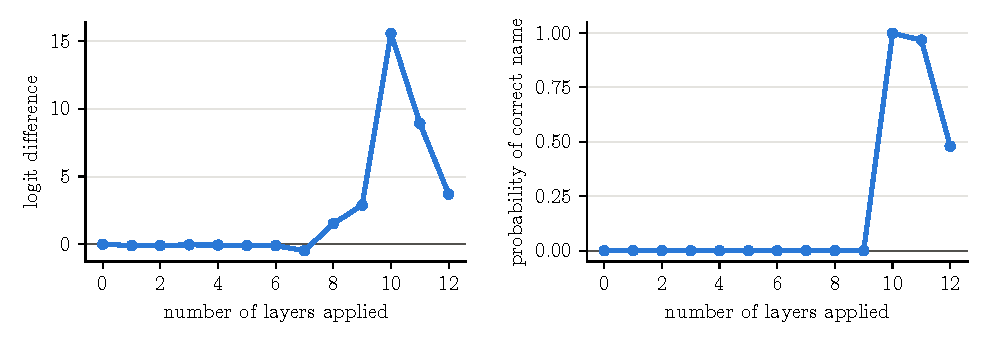
\includegraphics[width=0.82\textwidth]{figures/fig_logit_lens.pdf}
\caption{Logit lens on the IOI task in GPT-2 small, at the last position, averaged over 12 prompts. Left: lens
logit difference between the correct and the repeated name. Right: lens probability of the correct name. The
horizontal axis is the number $\ell$ of layers that have been applied, so $\ell=12$ is the real output.}
\label{fig:lens}
\end{figure}

\begin{caution}
The lens assumes that intermediate layers already use the output basis $W_U$. This is roughly true in late
layers and often false in early ones. The \emph{tuned lens} of \citet{belrose2023eliciting} relaxes the
assumption by training, for each layer, an affine map that is applied before the read-out. Magnitudes also need
care: $\LN$ in \eqref{eq:lens} rescales each intermediate stream by its own scale, so the height of the peak at
$\ell=10$ in \cref{fig:lens} is not on the scale of the final logits. Which layer makes the difference appear
is the robust part of the picture.
\end{caution}

\paragraph{Direct logit attribution.} The lens tells us \emph{when} the answer appears. \Cref{prop:dla} tells us
\emph{which component} wrote it. Applying \eqref{eq:dla} to the two tokens of \eqref{eq:ld} and subtracting gives
\begin{equation}\label{eq:dla-ld}
\logit_n(\mathrm{IO})-\logit_n(\mathrm{S}) \;=\; \sum_{g\in\mathcal G_n}
\frac{\big(W_U[\mathrm{IO}]-W_U[\mathrm{S}]\big)^\top\big(g-\mean(g)\,\one\big)}{\scale\big(x_n^{(L)}\big)} .
\end{equation}
Each summand is the \emph{direct logit attribution} (DLA) of one component: the amount by which this component,
through its own addition to the stream, moves the logit difference.

We computed all terms of \eqref{eq:dla-ld} for the running example. The terms add up to $3.7031$, and the logit
difference measured at the output is $3.7031$, as the proposition demands. The 144 heads together contribute
$3.45$, the 12 MLPs $0.25$, and the embeddings and bias terms less than $0.01$. \Cref{fig:dla} shows the heads.
Almost all of them contribute nothing. Four heads write clearly in favour of the correct name: 9.9
($+3.57$), 9.6 ($+1.10$), 10.6 ($+0.61$) and 10.0 ($+0.59$). Three of them are the heads whose attention patterns
we inspected in \cref{sec:attention}. Two heads write \emph{against} it: 10.7 ($-2.52$) and 11.10 ($-1.05$). They
sit in layers 10 and 11, which explains the drop after $\ell=10$ in \cref{fig:lens}.
\citet{wang2023interpretability} call 9.9, 9.6 and 10.0 \emph{name mover heads}, 10.6 a \emph{backup name mover
head}, and 10.7 and 11.10 \emph{negative name mover heads}.

\begin{figure}[t]
\centering
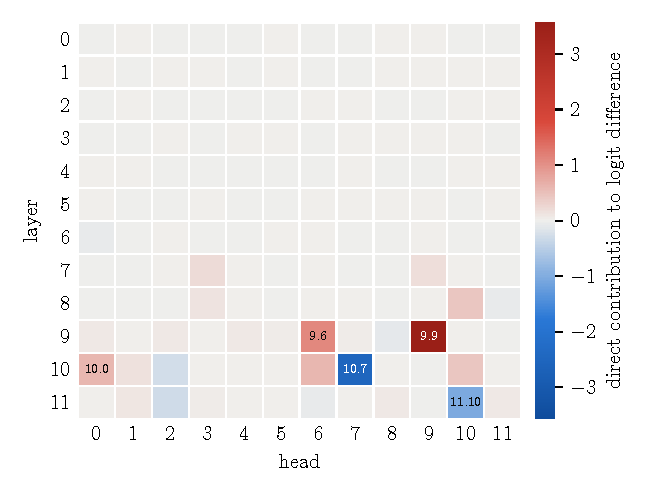
\includegraphics[width=0.5\textwidth]{figures/fig_dla_heads.pdf}
\caption{Direct logit attribution of each attention head of GPT-2 small to the logit difference of the IOI task
(summands of \eqref{eq:dla-ld}, averaged over 12 prompts). Red heads push towards the correct name and blue
heads push against it.}
\label{fig:dla}
\end{figure}

\begin{caution}
Equation \eqref{eq:dla-ld} is an exact accounting identity, and a DLA term is still not the effect of removing
the component. There are two reasons. The denominator $\scale(x_n^{(L)})$ depends on all components. And a
component also acts \emph{indirectly}, by changing what later components read. DLA sees only the direct path to
the output. A head in layer 5 that is essential for the task because head 9.9 depends on it can have a DLA of zero.
\Cref{sec:necessity} shows that this is exactly what happens in our example.
\end{caution}

\subsection{Probing}
\label{sec:probing}

The lens asks whether the \emph{answer} can be read from an intermediate activation. Probing asks the same
question for an arbitrary property \citep{alain2017understanding}. We collect a data set of pairs $(x,y)$,
where $x\in\R^d$ is an activation (say, the stream at a fixed layer and position) and $y\in\{0,1\}$ labels a
property of the input (say, whether the sentence is in the past tense). A \emph{linear probe} is a logistic
regression trained on these pairs,
\begin{equation}\label{eq:probe}
\Pr(y=1\mid x) \;=\; \frac{1}{1+\exp\!\big(-(w^\top x+b_{\mathrm{probe}})\big)},\qquad w\in\R^d,\ b_{\mathrm{probe}}\in\R .
\end{equation}
High accuracy on held-out data shows that the property is \emph{linearly decodable} from the activation.
Probes have found, among many other things, parts of speech and syntactic structure in the layers of BERT
\citep{tenney2019bert,hewitt2019structural} and the coordinates of places and the dates of events in the streams
of LLMs \citep{gurnee2024language}. \citet{belinkov2022probing} surveys the method.

A well-known case shows how much the choice of the property matters. \citet{li2023emergent} trained a
transformer to predict legal moves in the board game Othello from move sequences alone and asked whether the
state of the board can be decoded from its activations. Linear probes for the colour of each square (black,
white or empty) barely beat a baseline, and probes with one hidden layer succeeded. \citet{nanda2023emergent}
then found that a \emph{linear} probe works well once the question is rephrased relative to the player whose
turn it is: whether a square holds ``my'' piece or ``the opponent's''. The information was linear all along, in
a variable that the first study had not tried.

Three cautions govern the reading of any probing result.

\begin{enumerate}
\item \textbf{The probe may do the work itself.} A probe with enough capacity can learn the task from
any sufficiently rich input, whether or not the model has computed the property. \citet{hewitt2019designing}
propose \emph{control tasks}, in which each word type receives a random label. A good probe should reach high
accuracy on the real task and low accuracy on the control task, and the difference of the two accuracies is
called \emph{selectivity}. This is the reason for preferring linear probes: they have little capacity of their
own.
\item \textbf{Decodable does not mean used.} A probe establishes a correlation between an activation and a
label. The model may carry the information without ever reading it. To show that the model uses a direction,
we have to change the activation along it and observe the output, for example by erasing the direction
\citep{elazar2021amnesic} or by steering (\cref{sec:steering}).
\item \textbf{The probe direction need not be the model's direction.} Logistic regression chooses the $w$ that
separates the classes best, and it will exploit any other feature that happens to correlate with the label in
the data set. \citet{marks2024geometry} compare such directions with the plain difference between the two class
means and report that the latter is more often the one that changes the model's behaviour under intervention.
We return to this simple estimator in \cref{sec:lrh}.
\end{enumerate}

\begin{takeaways}
Attention patterns show from where a head reads and hide what it writes. Input attribution depends on a
baseline, and only integrated gradients are a true decomposition of the output change. The logit lens shows at
which layer an answer appears, and direct logit attribution shows which component wrote it, through the direct
path only. Probes show what is decodable, which is necessary and not sufficient for being used. In the running
example these tools point at layers 7 to 9, at the name mover heads 9.9, 9.6 and 10.0, and at the opposing heads
10.7 and 11.10.
\end{takeaways}

\begin{exercise}\label{ex:linearig}
Let $F$ be a linear function of $z$ without a constant term, so that its gradient $\nabla_{z_i}F$ is the same at
every point. Show that integrated gradients with baseline $\bar z=0$ coincide with gradient times input. Then take $n=d=1$ and $F(z)=z^2$, and show that
gradient times input is twice the integrated gradient.
\end{exercise}
\begin{exercise}\label{ex:lenslast}
Show that at $\ell=L$ the lens logits \eqref{eq:lens} are the logits of the model. Then explain why the sum of
the DLA terms of all components in layers $0,\dots,8$, together with the embeddings, is in general \emph{not}
equal to the lens logit difference at $\ell=9$.
\end{exercise}
\begin{exercise}\label{ex:probecontrol}
Suppose that a linear probe trained on the stream of layer 6 reaches 95\% accuracy for the property ``the
current token is a first name''. Describe a control experiment that shows whether this says anything
about layer 6, and predict its outcome using \eqref{eq:embed}.
\end{exercise}
